%!TEX root = ../thesis.tex
% ******************************* Thesis Appendix D ****************************

\chapter{MOSFET} 

MOSFETs (Metal-Oxide-Semiconductor Field-Effective Transistors) are the fundamental components of HV-MAPS technology. They apply the properties of p-n junctions to control the conductivity of a conduction channel between source and drain, through a gate-controlled external voltage.

The structure of a basic n-channel MOSFET (NMOS) is shown in Fig. \ref{img:MOSFET}. "N-channel" refers to the electron-conducting channel, which will be discussed in detailed later. There are 4 connections for a MOSFET: the source, drain, gate, and substrate. In a NMOS, the substrate is typically p-doped, while the source and drain are n-doped, creating two p-n junctions: between source-substrate and between substrate-drain. These junctions are oriented such that current cannot flow direcly from drain to source. In contrast, for a p-channel MOSFET (PMOS), the substrate is n-doped and the source \& drain are p-doped. 

\begin{figure}[h!] 
\centering
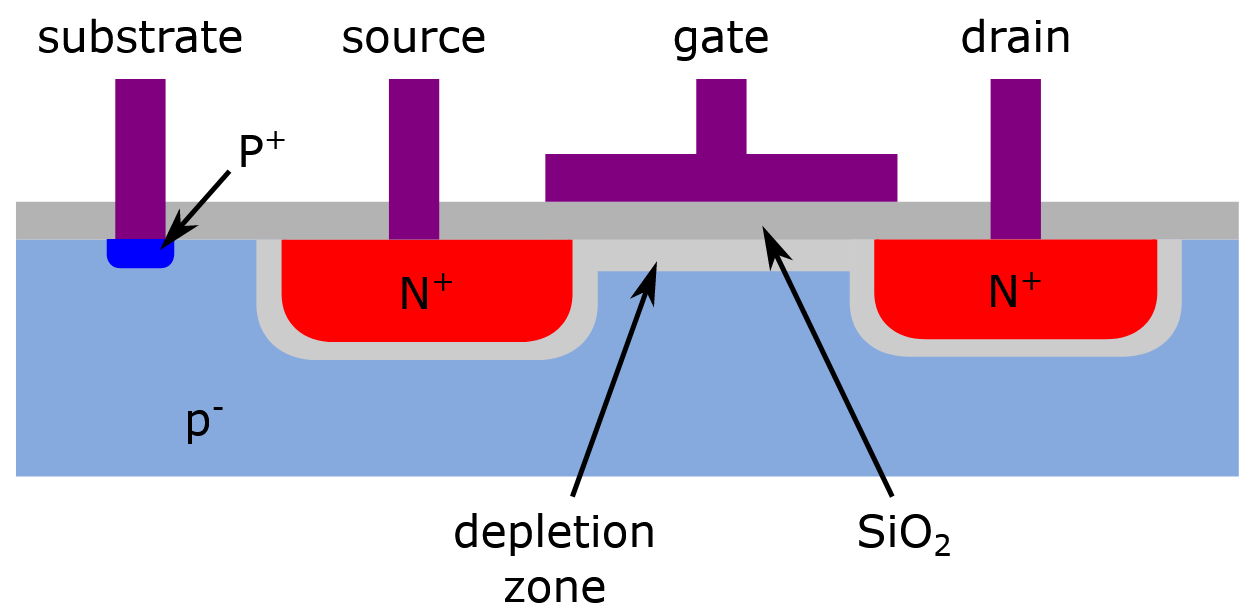
\includegraphics[width=0.65\linewidth]{Appendix4/MOSFET.png}
\caption{The sign on the doped regions refers to the concentration of doping\cite{Rudolf}.}
\label{img:MOSFET}
\end{figure}

The gate electrode is separated from the substrate by an insulating layer of silicon dioxide or ploy-silicon. 

When no voltage is applied to the gate, the source-drain current is negligible. The MOSFET is considered "off". 

When a positive gate voltage is applied (to NMOS), electrons in the p-doped substrate are attracted towards the interface between the substrate and the insulating layer. As the charge accumulates, a conduction channel begins to form between n-doped source and drain. At equilibrium, the the voltage of the accumulated carriers is equivalent to the gate voltage $V_{gs}$. Once $V_{gs}$ exceeds the threshold voltage $V_{th}$ - the voltage at which the number of free electrons equals to the number of holes in intrinsic silicon - an electron channel forms and source \& drain get electrically connected. The MOSFET is considered "on". Similar arguments with opposite doping applies to  p-channel MOSFET (PMOS)\footnote{For a PMOS, the substrate is n-doped and the minority carriers are the holes. When a negative gate voltage is applied, a hole-channel will be formed between the source and drain.}.

When the voltage between the source and the drain, $V_{ds}$, satisfies $V_{ds}<V_{gs}-V_{th}$, the MOSFET operates in the linear region. The conduction channel provides an ohmic connection, with current proportional to the voltage: $I_{ds} \propto V_{ds}$. When $V_{ds} = V_{gs}-V_{th}$, the channel pinched off at the drain. For $V_{ds} > V_{gs}-V_{th}$, the pinch-off point shifts towards the source, shortening the channel to compensate for the larger voltage. This marks the onset of the saturation region, where further increase in $V_{ds}$ have little effect on $I_{ds}$.

In summary, the conductivity between the source and drain of a MOSFET is controlled by gate voltage. The device acts as a voltage-controlled resistor in the linear region, and as voltage-controlled current source in saturation region.
